\documentclass{article}
\usepackage{microtype}
\usepackage{graphicx}
\usepackage{subcaption}
\usepackage{booktabs}
\usepackage{hyperref}
\usepackage{amsmath}
\usepackage{amssymb}
\usepackage{mathtools}
\usepackage{amsthm}
\usepackage[capitalize,noabbrev]{cleveref}
\usepackage{float}
\usepackage{needspace}
\usepackage{array}
\usepackage{tabularx}
\usepackage{multirow}
\newcolumntype{L}[1]{>{\raggedright\arraybackslash}p{#1}}
\newcolumntype{Y}{>{\raggedright\arraybackslash}X}
\usepackage[most]{tcolorbox}
\usepackage{tikz}
\usepackage{pgfplots}
\usetikzlibrary{positioning,calc,arrows.meta,fit,backgrounds}
\pgfplotsset{compat=1.18}
\graphicspath{{../figures/}}
\usepackage{icml2026}

% Tighten float and display spacing so the dense workshop paper does not
% strand large blank bands around figures, tables, and short equations.
\AtBeginDocument{%
  \setlength{\textfloatsep}{8pt plus 2pt minus 2pt}%
  \setlength{\floatsep}{7pt plus 2pt minus 2pt}%
  \setlength{\intextsep}{7pt plus 2pt minus 2pt}%
  \setlength{\abovecaptionskip}{4pt plus 1pt minus 1pt}%
  \setlength{\belowcaptionskip}{3pt plus 1pt minus 1pt}%
  \setlength{\abovedisplayskip}{5pt plus 2pt minus 2pt}%
  \setlength{\belowdisplayskip}{5pt plus 2pt minus 2pt}%
  \setlength{\abovedisplayshortskip}{3pt plus 1pt minus 1pt}%
  \setlength{\belowdisplayshortskip}{4pt plus 1pt minus 1pt}%
}

% Color definitions for figures
\definecolor{appleBlue}{RGB}{0, 122, 255}
\definecolor{appleLightBlue}{RGB}{235, 243, 255}
\definecolor{appleGreen}{RGB}{52, 199, 89}
\definecolor{appleLightGreen}{RGB}{238, 249, 239}
\definecolor{appleOrange}{RGB}{255, 149, 0}
\definecolor{appleLightOrange}{RGB}{255, 247, 235}
\definecolor{appleGray}{RGB}{142, 142, 147}
\definecolor{appleLightGray}{RGB}{242, 242, 247}
\definecolor{appleDark}{RGB}{28, 28, 30}
\definecolor{softTan}{RGB}{245,241,233}
\definecolor{softMint}{RGB}{236,245,240}

\icmltitlerunning{Transliteration ICL Failure Stages}
\newcommand{\papertitlepdf}{Early Entry, Late Drift: Stage-Specific Failure and Intervention in Multilingual Transliteration ICL}
\hypersetup{pdftitle={\papertitlepdf}}
\makeatletter
\newcommand{\forcerunningtitle}{\gdef\@icmltitlerunning{Transliteration ICL Failure Stages}}
\makeatother

\begin{document}
\twocolumn[
\icmltitle{\texorpdfstring{Early Entry, Late Drift:\\Stage-Specific Failure and Intervention\\in Multilingual Transliteration ICL}{\papertitlepdf}}
\forcerunningtitle
\begin{icmlauthorlist}
\icmlauthor{Anonymous Authors}{anon}
\end{icmlauthorlist}
\icmlaffiliation{anon}{Anonymous Institution}
\icmlcorrespondingauthor{Anonymous Authors}{anon@anon.invalid}
\icmlkeywords{mechanistic interpretability, multilingual in-context learning, transliteration}
\vskip 0.3in
]
\printAffiliationsAndNotice{}

%=====================================================================
% ABSTRACT - Using Farquhar's 5-sentence formula
%=====================================================================
\begin{abstract}
In-context learning (ICL) failures are often reported as a single accuracy drop, but Latin-to-Indic transliteration makes two failure stages visible: early target-entry failure and late prompt-bank continuation drift. We operationalize this split with first-akshara accuracy, continuation-tail CER, bank-copy diagnostics, and activation patching across five languages, then ask whether different stages expose different internal-state edit affordances. In \texttt{1B} Hindi, high-shot prompts often lose the first target token to Latin/source-like competitors; prompt-final patching identifies the strongest tested rescue at an \texttt{L25} MLP state, and a fixed two-channel shift gives a held-out rescue. In Telugu, a deliberately favorable shared-prefix oracle diagnostic identifies high-layer residual sites, yet the tested full-state mean-shift and Hindi-style compact-channel edits do not rescue continuation. Together, these results give a regime map plus one compact editable early-stage handle and one informative negative continuation-stage case; the Hindi edit reduces held-out CER from \textbf{0.827 to 0.703} ($n{=}200$), but we do not claim matched interventions or complete circuits.
\end{abstract}

%=====================================================================
% INTRODUCTION - Clear What/Why/So What structure
%=====================================================================
\section{Introduction}

When in-context learning fails, \emph{where} does it fail? A model can miss the correct target start entirely, or it can begin correctly and later drift toward a similar prompt exemplar. Those are different computational failures, not just different error severities, but many multilingual evaluations collapse them into one accuracy number.

We use multilingual transliteration to separate these stages. Transliteration exposes failure modes that are easy to tell apart: outputting Latin instead of the target script, starting correctly and then drifting toward a prompt-bank continuation, or producing the correct native-script word. Throughout the paper, the early axis is operationalized by \emph{first-akshara correctness}, not by a looser script-family check. This makes transliteration a useful setting for asking not only whether prompting helps, but which stage of the computation it helps or harms. The broader lesson is that ICL failure should not be treated as a scalar performance drop: different failure stages can expose different intervention affordances.

Our core empirical result is a behavioral regime map for 64-shot transliteration. The first axis is \emph{early target start}; the second is \emph{late query-specific continuation}. In Gemma~3 \texttt{1B}, Hindi fails early: helpful demonstrations worsen first-step competition and push output toward Latin. Telugu fails later: the model usually begins with the correct first akshara but then drifts toward similar prompt-bank continuations. Marathi, a same-script but different-language probe sharing Devanagari with Hindi, improves much more at the first akshara than at the continuation stage, though we do not treat it as a script-only control. In the broader figure-level summary, \texttt{4B} attenuates the clearest \texttt{1B} failures.

We then analyze two representative causal case studies inside that map. Under prompt-final alignment, Hindi's early failure concentrates in a candidate \texttt{L25} MLP causal handle, and a fixed two-channel edit derived from that handle improves held-out transliteration. Telugu instead points to a broader high-layer residual handle: the direct \texttt{1B} evidence centers on the post-\texttt{L25} residual, and a bounded \texttt{4B} follow-up identifies the post-\texttt{L33} residual as the strongest tested high-layer site. Yet even a shared-prefix-conditioned oracle diagnostic yields no comparable continuation rescue within the tested full-state mean-shift family. Because the Hindi and Telugu interventions are not a matched edit family, we treat this asymmetry as suggestive rather than definitive.

We deliberately keep the scope narrow. The paper's claim is not a universal theory of multilingual ICL. It is a multilingual transliteration regime map paired with two bounded causal case studies: one compact fixed edit and one informative negative intervention result.

Our contributions are threefold:
\begin{enumerate}
\item A \textbf{behavioral regime map for this transliteration setting} showing that 64-shot ICL failures separate into early-start versus late-continuation regimes (\S\ref{sec:behavior}).
\item \textbf{Causal diagnostics for two regimes}: Hindi points to a candidate compact near-output MLP handle, while Telugu points to broader high-layer residual handles, directly at the post-\texttt{L25} residual in \texttt{1B} and, in a bounded \texttt{4B} follow-up, most strongly at the post-\texttt{L33} residual (\S\ref{sec:mech}).
\item \textbf{Two bounded intervention outcomes}: a fixed two-channel Hindi patch reduces held-out CER from 0.827 to 0.703, while a Telugu shared-prefix-conditioned oracle mean-shift diagnostic yields no continuation rescue within the tested full-state edit family (\S\ref{sec:patch}, \S\ref{sec:bounds}).
\end{enumerate}

\begin{figure*}[t]
    \centering
    \begin{subfigure}[t]{0.48\textwidth}
        \centering
        \resizebox{\linewidth}{!}{% Static overview generated during final review polish.
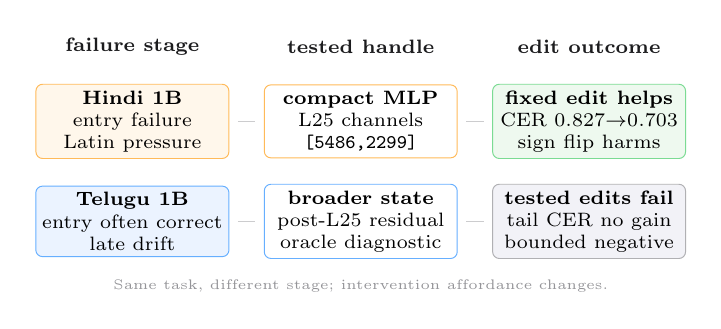
\begin{tikzpicture}[
  x=1cm,y=1cm,
  every node/.style={align=center},
  card/.style={rounded corners=2.4pt, line width=.35pt, minimum width=2.45cm, minimum height=.82cm, inner sep=2.3pt, font=\scriptsize},
  head/.style={font=\scriptsize\bfseries, text=appleDark},
  note/.style={font=\tiny, text=appleGray!95}
]
\node[head] at (1.28,3.10) {failure stage};
\node[head] at (4.18,3.10) {tested handle};
\node[head] at (7.08,3.10) {edit outcome};

\node[card, draw=appleOrange!65, fill=appleLightOrange] at (1.28,2.15)
  {\textbf{Hindi 1B}\\entry failure\\Latin pressure};
\node[card, draw=appleOrange!65, fill=white] at (4.18,2.15)
  {\textbf{compact MLP}\\L25 channels\\\texttt{[5486,2299]}};
\node[card, draw=appleGreen!65, fill=appleLightGreen] at (7.08,2.15)
  {\textbf{fixed edit helps}\\CER $0.827{\to}0.703$\\sign flip harms};

\node[card, draw=appleBlue!60, fill=appleLightBlue] at (1.28,0.88)
  {\textbf{Telugu 1B}\\entry often correct\\late drift};
\node[card, draw=appleBlue!60, fill=white] at (4.18,0.88)
  {\textbf{broader state}\\post-L25 residual\\oracle diagnostic};
\node[card, draw=appleGray!70, fill=appleLightGray] at (7.08,0.88)
  {\textbf{tested edits fail}\\tail CER no gain\\bounded negative};

\draw[appleGray!45,line width=.35pt] (2.62,2.15) -- (2.84,2.15);
\draw[appleGray!45,line width=.35pt] (5.52,2.15) -- (5.74,2.15);
\draw[appleGray!45,line width=.35pt] (2.62,0.88) -- (2.84,0.88);
\draw[appleGray!45,line width=.35pt] (5.52,0.88) -- (5.74,0.88);

\node[note] at (4.18,0.06)
  {Same task, different stage; intervention affordance changes.};
\path[use as bounding box] (-0.05,-0.10) rectangle (8.40,3.34);
\end{tikzpicture}
}
        \caption{The two case studies connect failure stage, tested state handle, and intervention outcome.}
        \label{fig:stage_intervention_overview}
    \end{subfigure}\hfill
    \begin{subfigure}[t]{0.48\textwidth}
        \centering
        \resizebox{\linewidth}{!}{% Auto-generated by experiments/render_stage_axis_map.py
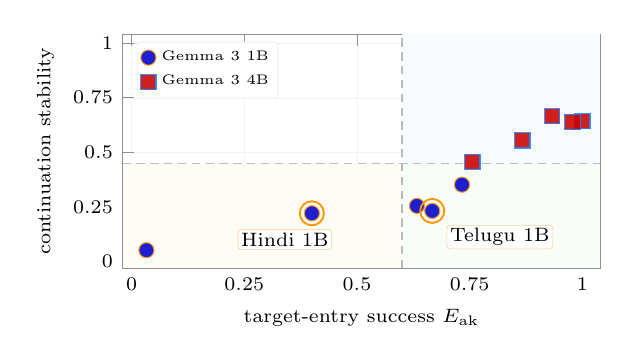
\begin{tikzpicture}
\begin{axis}[width=7.65cm,height=4.55cm,xmin=-0.02,xmax=1.04,ymin=-0.03,ymax=1.04,xlabel={target-entry success $E_{\mathrm{ak}}$},ylabel={continuation stability},xtick={0,0.25,0.5,0.75,1.0},ytick={0,0.25,0.5,0.75,1.0},grid=major,major grid style={line width=.16pt,draw=appleLightGray},axis line style={draw=appleGray},tick style={draw=appleGray},label style={font=\scriptsize},tick label style={font=\scriptsize},clip=false,legend style={draw=appleLightGray,fill=white,fill opacity=0.94,text opacity=1,font=\tiny,at={(0.03,0.97)},anchor=north west,rounded corners=1pt,inner sep=1.2pt},legend cell align={left}]
\fill[appleOrange!4] (axis cs:-0.02,-0.03) rectangle (axis cs:0.60,0.45);
\fill[appleBlue!3] (axis cs:0.60,0.45) rectangle (axis cs:1.04,1.04);
\fill[appleGreen!3] (axis cs:0.60,-0.03) rectangle (axis cs:1.04,0.45);
\draw[densely dashed,appleGray!60,line width=.42pt] (axis cs:0.60,-0.03) -- (axis cs:0.60,1.04);
\draw[densely dashed,appleGray!60,line width=.42pt] (axis cs:-0.02,0.45) -- (axis cs:1.04,0.45);
\addplot+[only marks,mark=*,mark size=2.75pt,draw=appleOrange!90,fill=appleOrange!78,opacity=0.88] coordinates {(0.400,0.221) (0.733,0.352) (0.033,0.052) (0.633,0.255) (0.667,0.232)};
\addlegendentry{Gemma 3 1B}
\addplot+[only marks,mark=square*,mark size=2.75pt,draw=appleBlue!90,fill=appleBlue!78,opacity=0.88] coordinates {(0.867,0.555) (0.933,0.665) (0.756,0.457) (1.000,0.643) (0.978,0.639)};
\addlegendentry{Gemma 3 4B}
\addplot+[only marks,mark=o,mark size=4.35pt,draw=appleOrange,line width=.68pt] coordinates {(0.400,0.221)};
\node[font=\scriptsize,fill=white,fill opacity=0.96,text opacity=1,inner sep=1.15pt,rounded corners=1pt,draw=appleOrange!45,line width=.22pt] at (axis cs:0.340,0.101) {Hindi 1B};
\addplot+[only marks,mark=o,mark size=4.35pt,draw=appleOrange,line width=.68pt] coordinates {(0.667,0.232)};
\node[font=\scriptsize,fill=white,fill opacity=0.96,text opacity=1,inner sep=1.15pt,rounded corners=1pt,draw=appleOrange!45,line width=.22pt] at (axis cs:0.817,0.112) {Telugu 1B};
\end{axis}
\end{tikzpicture}
}
        \caption{A data-driven stage map separates early target entry from continuation stability.}
        \label{fig:axes}
    \end{subfigure}
    \caption{\textbf{Paper overview.} Transliteration exposes ICL failures as stage-specific errors, and the Hindi/Telugu case studies show that different stages can have different intervention affordances.}
    \label{fig:teaser}
\end{figure*}

%=====================================================================
% TASK, DATA, AND MEASUREMENTS
%=====================================================================
\section{Task, Data, and Measurements}\label{sec:task}

We study Latin-to-native-script transliteration for five Indic languages: Hindi and Marathi (Devanagari), Telugu (Telugu script), Tamil (Tamil script), and Bengali (Bengali script), using Aksharantar \citep{aksharantar}. Unless otherwise stated, prompts contain $k{=}64$ source-target demonstrations $((x_1,y_1),\ldots,(x_k,y_k))$ followed by a held-out query $x_q$, and the model must generate the native-script target $y_q$. The query split is held out from the prompt bank. This task is useful because early target-start failure, late prompt-bank drift, and successful composition are easy to distinguish behaviorally.

We compare three conditions. \textbf{Helpful} uses correct $(x_i,y_i)$ pairs. \textbf{Corrupt} randomly permutes targets, preserving format and target-token statistics while removing semantic alignment. \textbf{Zero-shot} uses no demonstrations. Helpful-versus-zero-shot defines the main multilingual regime map; corrupt is used more selectively as a supporting control when we need to ask whether an effect depends on semantic alignment rather than prompt state alone.

Our main metrics are as follows. \textbf{Exact match (EM)} is strict string equality after NFC normalization. \textbf{Akshara CER} is Levenshtein error over orthographic syllables rather than raw Unicode characters:
\begin{equation}
\mathrm{CER} = \frac{\mathrm{Levenshtein}(A_{\hat y},A_{y^*})}{\max(1,|A_{y^*}|)},
\end{equation}
where $A_y$ is the akshara sequence of $y$. \textbf{First-akshara correctness} $E_{\mathrm{ak}}$ is the paper's operational early-stage metric. \textbf{Continuation-tail CER} $\mathrm{CER}_{\mathrm{tail}}$ is computed on the suffix after the first akshara, conditioned on a correct first akshara; when the gold suffix is empty, the implementation assigns tail CER $0$ if no extra tail is produced and $1$ otherwise. \textbf{First-token target rate} $E_{\mathrm{tok}}$ and the \textbf{target-vs-majority-Latin/ASCII logit gap} $\Delta \mathcal{L}$ are used only in the Hindi causal analyses, where the intervention acts directly on first-step logits. \textbf{Bank-copy rate} tracks exact prompt-exemplar copying. For Telugu, we also use a \textbf{nearest-bank competitor} chosen by source-side \texttt{SequenceMatcher} similarity, a \textbf{fuzzy bank-copy} threshold of $0.85$, and a \textbf{first-divergence gold-vs-bank gap} $\Delta \mathcal{L}_{\mathrm{div}}$ measured at the first token where the gold continuation and the selected competitor diverge. We treat $\Delta \mathcal{L}_{\mathrm{div}}$ as a single-competitor diagnostic, not as a competitor-agnostic measure of all bank-attractor pressure.

We analyze instruction-tuned Gemma~3 \texttt{1B} and \texttt{4B} \citep{gemma3report} with greedy decoding unless stated otherwise. Hindi, Bengali, Tamil, and Telugu cells in the broad behavioral summary aggregate seeds $\{11,42,101\}$; Marathi appears there only as a targeted seed-42 same-script diagnostic. Mechanistic and intervention panels use narrower seed-42 splits, with separate selection and evaluation panels for the held-out patch results. Confidence intervals are nonparametric bootstrap intervals over evaluation items. For implementation clarity, we refer to the Hindi site as the \texttt{L25} MLP state, the main Telugu \texttt{1B} site as the post-\texttt{L25} residual, and the strongest tested Telugu \texttt{4B} follow-up site as the post-\texttt{L33} residual; Appendix Table~\ref{tab:panelsummary} summarizes the panel roles. Table~\ref{tab:claimledger} states the claims and limits that the rest of the paper must support.

\begin{table*}[t]
\centering
\begingroup
\footnotesize
\setlength{\tabcolsep}{5pt}
\renewcommand{\arraystretch}{1.08}
\begin{tabularx}{\textwidth}{L{3.2cm}YY}
\toprule
\textbf{Claim and status} & \textbf{Primary evidence} & \textbf{Main limitation} \\
\midrule
\textbf{C1: Stage separation}\par\emph{established} & Fig.~\ref{fig:behavior} and Table~\ref{tab:axes_metrics}: first-akshara correctness, continuation-tail CER, and bank-copy move differently across languages and scale & broad map uses small per-seed panels; Marathi is seed-42 only \\
\textbf{C2: Compact Hindi handle}\par\emph{supported, bounded} & prompt-final patching peaks at \texttt{L25} MLP; channel selection repeatedly isolates \texttt{[5486,2299]}; held-out fixed patch improves CER & same-length helpful/corrupt patching finds a broader layer-output content signal rather than reproducing the compact \texttt{L25} MLP rescue \\
\textbf{C3: Telugu residual diagnostic}\par\emph{supported as diagnostic} & donor replacement at post-\texttt{L25} in \texttt{1B} and post-\texttt{L33} in \texttt{4B} improves the gold-vs-bank divergence gap over off-band/random controls & writer-head evidence is exploratory and bank-copy is only one late-drift proxy \\
\textbf{C4: No Telugu rescue}\par\emph{established for tested edit} & shared-prefix-conditioned oracle mean-shift leaves continuation exact match at 0 and does not improve continuation CER on 191 usable items & not a proof that Telugu continuation failures are intrinsically uneditable \\
\bottomrule
\end{tabularx}
\endgroup
\caption{\textbf{Claim ledger.} We separate observed behavior, causal diagnostics, intervention results, and limitations so the mechanistic contrast is not stronger than the evidence.}
\label{tab:claimledger}
\vspace{4pt}
\end{table*}

%=====================================================================
% BEHAVIORAL REGIME MAP
%=====================================================================
\section{Behavioral Regime Map}\label{sec:behavior}

\subsection{Distinct Failure Regimes}

Figure~\ref{fig:behavior} compares helpful prompting with zero-shot. The main result is that Gemma~3 \texttt{1B} does not fail uniformly: different language cells land in different algorithmic regimes.

\textbf{Hindi} has an early routing failure: helpful ICL lowers exact match, worsens CER, and shifts first-step competition toward Latin and source-like competitors. \textbf{Telugu} differs: the model usually begins with the correct first akshara and then drifts toward prompt-bank continuations. The dominant competition is therefore later, between the gold continuation and a nearby prompt-bank attractor rather than between target script and Latin. \textbf{Marathi}, our same-script different-language probe, improves much more at the first akshara than at continuation; we use it as targeted diagnostic support rather than as a script-only control or a second full causal case study.

Across the remaining broad-map cells, \textbf{Bengali} remains weak in \texttt{1B}, while \textbf{Tamil} improves more reliably in \texttt{4B}. \textbf{Marathi} appears there only as a targeted seed-42 row rather than a three-seed estimate, so the five-language figure should be read as a broad phase map rather than a full stage-resolved ranking.

\begin{figure*}[t]
    \centering
    \resizebox{0.98\textwidth}{!}{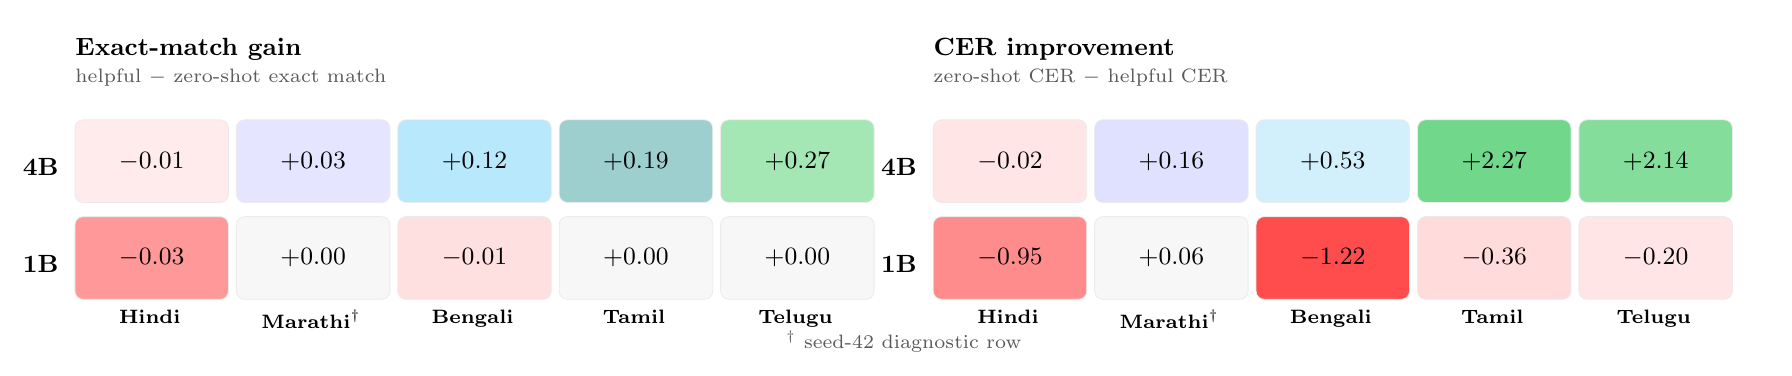
\begin{tikzpicture}[x=1cm,y=1cm, every node/.style={inner sep=0pt}]
  \def\cellw{1.95}
  \def\cellh{1.05}
  \def\leftx{0}
  \def\rightx{10.9}

  \tikzset{
    cell/.style={draw=black!8, line width=0.3pt, rounded corners=3pt},
    head/.style={font=\bfseries\small},
    collab/.style={font=\bfseries\scriptsize},
    num/.style={font=\bfseries\small},
    tinycap/.style={font=\scriptsize, text=black!65}
  }

  % enlarge the effective bounding box so the bottom labels are never clipped by the caption
  \path[use as bounding box] (\leftx-0.6, -3.25) rectangle (\rightx+10.55, 0.82);

  % panel titles
  \node[anchor=west, head] at (\leftx, 0.55) {Exact-match gain};
  \node[anchor=west, tinycap] at (\leftx, 0.18) {helpful $-$ zero-shot exact match};
  \node[anchor=west, head] at (\rightx, 0.55) {CER improvement};
  \node[anchor=west, tinycap] at (\rightx, 0.18) {zero-shot CER $-$ helpful CER};

  % row labels
  \node[anchor=east, head] at (\leftx-0.2, -0.95) {4B};
  \node[anchor=east, head] at (\leftx-0.2, -2.18) {1B};
  \node[anchor=east, head] at (\rightx-0.2, -0.95) {4B};
  \node[anchor=east, head] at (\rightx-0.2, -2.18) {1B};

  % column labels are drawn after the cells so they cannot be occluded by the heatmap blocks

  % left panel, 4B
  \path[fill=red!8!white, cell] (\leftx+0.00, -0.35) rectangle ++(\cellw,-\cellh);
  \node[num] at (\leftx+0.975, -0.875) {$-0.01$};
  \path[fill=blue!10!white, cell] (\leftx+2.05, -0.35) rectangle ++(\cellw,-\cellh);
  \node[num] at (\leftx+3.025, -0.875) {$+0.03$};
  \path[fill=cyan!28!white, cell] (\leftx+4.10, -0.35) rectangle ++(\cellw,-\cellh);
  \node[num] at (\leftx+5.075, -0.875) {$+0.12$};
  \path[fill=teal!38!white, cell] (\leftx+6.15, -0.35) rectangle ++(\cellw,-\cellh);
  \node[num] at (\leftx+7.125, -0.875) {$+0.19$};
  \path[fill=appleGreen!45!white, cell] (\leftx+8.20, -0.35) rectangle ++(\cellw,-\cellh);
  \node[num] at (\leftx+9.175, -0.875) {$+0.27$};

  % left panel, 1B
  \path[fill=red!40!white, cell] (\leftx+0.00, -1.58) rectangle ++(\cellw,-\cellh);
  \node[num] at (\leftx+0.975, -2.105) {$-0.03$};
  \path[fill=black!3, cell] (\leftx+2.05, -1.58) rectangle ++(\cellw,-\cellh);
  \node[num] at (\leftx+3.025, -2.105) {$+0.00$};
  \path[fill=red!12!white, cell] (\leftx+4.10, -1.58) rectangle ++(\cellw,-\cellh);
  \node[num] at (\leftx+5.075, -2.105) {$-0.01$};
  \path[fill=black!3, cell] (\leftx+6.15, -1.58) rectangle ++(\cellw,-\cellh);
  \node[num] at (\leftx+7.125, -2.105) {$+0.00$};
  \path[fill=black!3, cell] (\leftx+8.20, -1.58) rectangle ++(\cellw,-\cellh);
  \node[num] at (\leftx+9.175, -2.105) {$+0.00$};

  % right panel, 4B
  \path[fill=red!10!white, cell] (\rightx+0.00, -0.35) rectangle ++(\cellw,-\cellh);
  \node[num] at (\rightx+0.975, -0.875) {$-0.02$};
  \path[fill=blue!12!white, cell] (\rightx+2.05, -0.35) rectangle ++(\cellw,-\cellh);
  \node[num] at (\rightx+3.025, -0.875) {$+0.16$};
  \path[fill=cyan!18!white, cell] (\rightx+4.10, -0.35) rectangle ++(\cellw,-\cellh);
  \node[num] at (\rightx+5.075, -0.875) {$+0.53$};
  \path[fill=appleGreen!70!white, cell] (\rightx+6.15, -0.35) rectangle ++(\cellw,-\cellh);
  \node[num] at (\rightx+7.125, -0.875) {$+2.27$};
  \path[fill=appleGreen!60!white, cell] (\rightx+8.20, -0.35) rectangle ++(\cellw,-\cellh);
  \node[num] at (\rightx+9.175, -0.875) {$+2.14$};

  % right panel, 1B
  \path[fill=red!45!white, cell] (\rightx+0.00, -1.58) rectangle ++(\cellw,-\cellh);
  \node[num] at (\rightx+0.975, -2.105) {$-0.95$};
  \path[fill=black!3, cell] (\rightx+2.05, -1.58) rectangle ++(\cellw,-\cellh);
  \node[num] at (\rightx+3.025, -2.105) {$+0.06$};
  \path[fill=red!70!white, cell] (\rightx+4.10, -1.58) rectangle ++(\cellw,-\cellh);
  \node[num] at (\rightx+5.075, -2.105) {$-1.22$};
  \path[fill=red!14!white, cell] (\rightx+6.15, -1.58) rectangle ++(\cellw,-\cellh);
  \node[num] at (\rightx+7.125, -2.105) {$-0.36$};
  \path[fill=red!10!white, cell] (\rightx+8.20, -1.58) rectangle ++(\cellw,-\cellh);
  \node[num] at (\rightx+9.175, -2.105) {$-0.20$};

  % column labels
  \node[anchor=north, collab] at (\leftx+0.95, -2.76) {Hindi};
  \node[anchor=north, collab] at (\leftx+3.00, -2.76) {Marathi$^{\dagger}$};
  \node[anchor=north, collab] at (\leftx+5.05, -2.76) {Bengali};
  \node[anchor=north, collab] at (\leftx+7.10, -2.76) {Tamil};
  \node[anchor=north, collab] at (\leftx+9.15, -2.76) {Telugu};

  \node[anchor=north, collab] at (\rightx+0.95, -2.76) {Hindi};
  \node[anchor=north, collab] at (\rightx+3.00, -2.76) {Marathi$^{\dagger}$};
  \node[anchor=north, collab] at (\rightx+5.05, -2.76) {Bengali};
  \node[anchor=north, collab] at (\rightx+7.10, -2.76) {Tamil};
  \node[anchor=north, collab] at (\rightx+9.15, -2.76) {Telugu};

  \node[anchor=north, tinycap] at ({0.5*(\leftx+\rightx+10.15)}, -3.02) {$^{\dagger}$ seed-42 diagnostic row};

\end{tikzpicture}
}
    \caption{\textbf{Gemma~3 \texttt{1B} splits into distinct failure regimes; \texttt{4B} attenuates the clearest ones.} Left: EM gain from helpful ICL. Right: CER reduction, where positive values mean helpful beats zero-shot and values above 1 can occur under severe zero-shot overgeneration. Hindi, Bengali, Tamil, and Telugu are three-seed means over $\{11,42,101\}$; Marathi$^{\dagger}$ is a targeted seed-42 same-script diagnostic. Table~\ref{tab:axes_metrics} reports the stage-sensitive axes used for the regime interpretation.}
    \label{fig:behavior}
\end{figure*}

\begin{table}[t]
\centering
\small
\setlength{\tabcolsep}{4.5pt}
\begin{tabular}{@{}lccc@{}}
\toprule
\textbf{1B, $k{=}64$} & \textbf{$E_{\mathrm{ak}}$} & \textbf{$\mathrm{CER}_{\mathrm{tail}}$} & \textbf{Bank copy} \\
 & \textbf{zs$\to$help} & \textbf{help ($n$)} & \textbf{help} \\
\midrule
Hindi   & $0.60 \to 0.50$ & 0.75 (15) & 0.27 \\
Marathi & $0.37 \to 0.73$ & 0.65 (22) & 0.37 \\
Telugu  & $0.00 \to 0.90$ & 0.67 (27) & 0.80 \\
\bottomrule
\end{tabular}
\caption{\textbf{Stage-sensitive evidence for the two axes.} $E_{\mathrm{ak}}$ is first-akshara correctness. $\mathrm{CER}_{\mathrm{tail}}$ is helpful-condition continuation-tail CER conditioned on a correct first akshara; parentheses give eligible counts. Bank copy is exact prompt-bank copying. Rows use matched 30-item seed-42 diagnostic panels.}
\label{tab:axes_metrics}
\vspace{4pt}
\end{table}

Table~\ref{tab:axes_metrics} shows the regime split directly. In Hindi, helpful prompting degrades both end-to-end quality and first-akshara correctness. In Marathi, the first akshara improves sharply but continuation-tail CER remains high. In Telugu, the first akshara is usually correct, yet continuation-tail CER remains 0.67 and exact bank-copy reaches 0.80. Throughout the rest of the paper, we treat $\mathrm{CER}_{\mathrm{tail}}$ as the direct late-axis metric and bank-copy as a narrower proxy for one prompt-bank failure mode.

\subsection{K-shot Scaling Supports the Decomposition}\label{sec:kshot}

A fixed-split single-seed 60-item sweep over $k \in \{8,16,32,64,128\}$ supports the same decomposition (Appendix~\ref{app:kshot}, Table~\ref{tab:kshot}). Hindi is strongest around $k{=}32$ before degrading again at $k{=}64$ and $128$. Telugu behaves differently: exact helpful bank-copy rises sharply at $k{=}64$, and when we condition on a correct first akshara in the stored item-level outputs, the exact bank-copy rate still rises from roughly $0.40$ at $k{=}16/32$ to $0.74$ at $k{=}64$ before falling at $k{=}128$ (eligible counts $20/25/31/25$ for $k{=}16/32/64/128$). We therefore treat the sweep as supportive evidence that prompt mass can strengthen a late attractor rather than helping monotonically.

These behavioral results motivate different mechanistic hypotheses. Hindi resembles an early target-start problem, so a compact near-output causal handle is plausible. Telugu is continuation-limited, so a broader state after the first akshara is the natural target. We test both hypotheses next.

%=====================================================================
% CAUSAL DIAGNOSTICS AND INTERVENTIONS
%=====================================================================
\section{Causal Diagnostics and Interventions}\label{sec:mech}

The behavioral regimes suggest different causal-handle hypotheses. We test where targeted activation changes move the relevant logits and whether those changes yield fixed interventions.

\subsection{Hindi: Candidate Compact MLP Handle}

This subsection uses the auxiliary metric $E_{\mathrm{tok}}$, the first-token target rate at the \emph{tokenizer} level, because the causal intervention acts directly on pre-generation logits. On the 200-item held-out Hindi patch panel used later, $E_{\mathrm{tok}}$ and akshara-level first-entry agree on 167/200 items (83.5\%). The bridge is imperfect but meaningful: the itemwise correlation between patch-induced $\Delta \mathcal{L}$ and itemwise change in first-entry correctness is $0.40$, and among the 119 baseline first-entry failures, the 51 rescued items show larger mean $\Delta \mathcal{L}$ improvement than the 68 non-rescued failures ($+8.26$ versus $+5.65$).

Hindi's failure is concentrated at the first token. $E_{\mathrm{tok}}$ falls from $0.60$ in zero-shot to $0.47$ under helpful prompting, and Latin outputs become common. Corrupt prompts are similarly harmful ($E_{\mathrm{tok}}{=}0.43$; Latin top-1 on $56.7\%$ of items versus $50.0\%$ under helpful), which argues against a purely semantic retrieval story.

We localize the helpful-versus-zero-shot contrast with prompt-final activation patching \citep{patchingbest, rome}:
\begin{equation}
\tilde{h}^{\mathrm{help}}_{l,p_{\mathrm{help}}} \leftarrow h^{\mathrm{zs}}_{l,p_{\mathrm{zs}}}.
\end{equation}
Only the chosen layer-position activation is transplanted. Because helpful and zero-shot prompts differ strongly in absolute length, this is prompt-final alignment. On the 30-item sweep, helpful$\leftarrow$zero-shot patching at the \texttt{L25} MLP output gives the largest mean target-vs-majority-Latin/ASCII gap improvement ($+3.30$), ahead of \texttt{L23 layer\_output} ($+2.58$) and \texttt{L20 layer\_output} ($+2.51$). A matched same-length helpful/corrupt patch sweep does not reproduce this compact \texttt{L25} MLP rescue: corrupt$\leftarrow$helpful peaks instead at \texttt{L23 layer\_output} ($+2.37$), while helpful$\leftarrow$corrupt is small and leaves top-1 target rate unchanged (Appendix Table~\ref{tab:hindi_same_length}). We therefore read the \texttt{L25} MLP result as a compact high-shot prompt-state competition handle, not as a clean semantic helpful-vs-corrupt retrieval site.

Within that block, the later channel ranking and deployed patch move one step inward to the 6912-dimensional pre-down-projection channel basis captured at \texttt{mlp.down\_proj}. A strict selection$\to$evaluation pipeline isolates a small negative-signed family whose held-out repeat-seed check independently re-selects the same two-channel core, \texttt{[5486,2299]}, with a $+4.004$ logit-gap improvement over matched random-channel controls. We do not give these channels semantic names. The minimal interpretation is readout-geometric: helpful high-shot prompts increase both coordinates relative to zero-shot, and the local down-projection/readout geometry makes shifting them back toward zero-shot increase the gold-first-token-vs-Latin margin (Appendix Table~\ref{tab:hindi_channel_readout}). An item-level audit supports the same bounded view, not a clean monosemantic label: channel 2299 is more associated with Latin top-1 pressure, while channel 5486 appears in both base-success and Latin-collapse contexts. Taken together, the Hindi case is compact both behaviorally and implementationally: the dominant problem is early, and much of the harmful high-shot shift is captured by a small basis inside one near-output MLP state.

\subsection{Telugu: Broader Residual Diagnostic}

On the matched 30-item helpful panel, Telugu usually gets the first akshara right and then drifts toward prompt-bank continuations. The nearest-bank heuristic is not a complete account of what gets copied, but exact bank copies on the 30-item diagnostic are still concentrated near the top of both the source-side and target-side similarity rankings, so the late attractor signal is real rather than an artifact of one arbitrary comparison word.

A separate 57-item helpful follow-up shows that this attractor survives stochastic decoding: sample-level exact bank-copy rises from $0.42$ at $T{=}0.0$ to $0.50$ at $T{=}0.2$ and $0.59$ at $T{=}0.7$, with fuzzy bank-copy rising from $0.47$ to $0.55$ to $0.64$ (Appendix~\ref{app:tempsweep}, Table~\ref{tab:tempsweep}). The main mechanistic donor-replacement result is later and broader than Hindi's. In \texttt{1B}, the directly demonstrated site is the post-\texttt{L25} residual. A bounded \texttt{4B} residual-site follow-up identifies the post-\texttt{L33} residual as the strongest tested high-layer site, raising the mean first-divergence gold-vs-bank gap by $+9.10$ on a 57-item panel versus $+4.30$ at off-band \texttt{L20}. Appendix~\ref{app:telugu_followups} also reports exploratory writer-head screens: the strongest \texttt{1B} heads cluster around \texttt{L18}, whereas \texttt{4B}'s strongest heads are later and more distributed. We treat those head-level results as hypothesis-generating.

This contrast with Hindi matters. The Telugu evidence is not a null localization result: high-layer residual interventions move the diagnostic divergence gap in the tested panels. What is missing is transfer to a simple fixed edit. The handle is broader, later, and more state-like, which may help explain why diagnosis is easier than repair.

%=====================================================================
% HELD-OUT INTERVENTIONS
%=====================================================================
\section{Held-Out Interventions}\label{sec:patch}

\subsection{Hindi: Fixed Patch Transfers}

We test whether the Hindi mechanism supports a fixed inference-time intervention. Within that same \texttt{L25} block, let $c_{25,p} \in \mathbb{R}^{6912}$ denote the post-gating, pre-down-projection MLP channel vector at the last prompt position $p$; in code, this is the tensor captured by a forward pre-hook on \texttt{mlp.down\_proj}. For the selected channel set $S = \{5486,2299\}$, the deployed patch updates only those coordinates: $c'_S = c_S + \alpha(\bar c^{\mathrm{zs}}_S - \bar c^{\mathrm{help}}_S)$, where $c_S$ abbreviates $c_{25,p,S}$ and all coordinates outside $S$ are unchanged. The means $\bar c^{\mathrm{zs}}_S$ and $\bar c^{\mathrm{help}}_S$ are computed on the disjoint selection split: for each item $i$, we extract the channel vector at that item's own prompt-final position $p^{(i)}$, then average across items. Thus $\bar c^{\mathrm{zs}}_S = \frac{1}{N}\sum_i c^{\mathrm{zs},(i)}_{25,p^{(i)}_{\mathrm{zs}},S}$, with the helpful mean defined analogously. This 200-item $\alpha$-tuning panel is separate from the 100-item channel-selection split used in \S\ref{sec:mech}. For the practical patch, we tune $\alpha$ by maximizing the mean first-step target-vs-majority-Latin/ASCII gap $\Delta \mathcal{L}$ on that 200-item selection split, using the mean gold first-token probability $p_{\mathrm{target}}$ (the model probability assigned to the gold first token) only as a tie-break; the deployed patch uses $\alpha=2.0$. Figure~\ref{fig:hpatch}A also reports $\Delta p_{\mathrm{target}}$, the patch-induced change in that same mean gold first-token probability. The sign-flip baseline applies the negative of the same shift, and the zero-ablate baseline sets $c_{25,p,S}=0$ at the same site. We then evaluate the chosen patch unchanged on a disjoint 200-item held-out panel.

\begin{figure}[t]
    \centering
    \resizebox{\linewidth}{!}{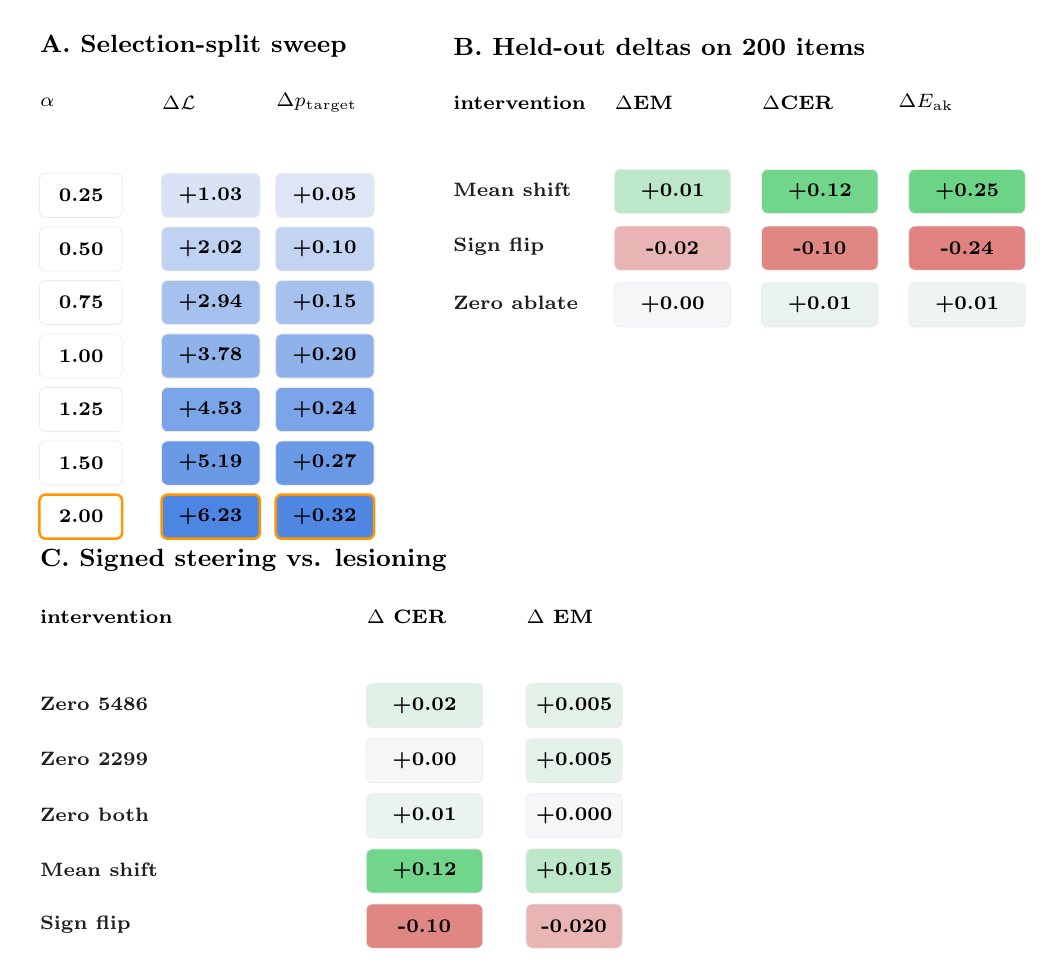
\begin{tikzpicture}[x=1cm,y=1cm, every node/.style={inner sep=0pt}]
  \tikzset{cell/.style={draw=black!8, line width=0.28pt, rounded corners=2.2pt}, head/.style={font=\bfseries\small}, rowlab/.style={font=\bfseries\scriptsize, text=black!88}, colab/.style={font=\bfseries\scriptsize}, tinycap/.style={font=\scriptsize, text=black!63}, num/.style={font=\bfseries\scriptsize}}

  \node[anchor=west, head] at (0.0,0.38) {A. Selection-split sweep};
  \node[anchor=west, colab] at (0.00,-0.33) {$\alpha$};
  \node[anchor=west, colab] at (1.55,-0.33) {$\Delta \mathcal{L}$};
  \node[anchor=west, colab] at (3.00,-0.33) {$\Delta p_{\mathrm{target}}$};
  \definecolor{hpA_gap_0}{RGB}{218,227,245}
  \definecolor{hpA_prob_0}{RGB}{222,230,246}
  \path[fill=white, draw=black!8, line width=0.28pt, rounded corners=2.2pt] (0.00,-1.23) rectangle ++(1.05,-0.56);
  \node[num] at (0.53,-1.51) {0.25};
  \path[fill=hpA_gap_0, draw=black!8, line width=0.28pt, rounded corners=2.2pt] (1.55,-1.23) rectangle ++(1.25,-0.56);
  \node[num] at (2.17,-1.51) {+1.03};
  \path[fill=hpA_prob_0, draw=black!8, line width=0.28pt, rounded corners=2.2pt] (3.00,-1.23) rectangle ++(1.25,-0.56);
  \node[num] at (3.62,-1.51) {+0.05};
  \definecolor{hpA_gap_1}{RGB}{191,210,242}
  \definecolor{hpA_prob_1}{RGB}{195,212,242}
  \path[fill=white, draw=black!8, line width=0.28pt, rounded corners=2.2pt] (0.00,-1.91) rectangle ++(1.05,-0.56);
  \node[num] at (0.53,-2.19) {0.50};
  \path[fill=hpA_gap_1, draw=black!8, line width=0.28pt, rounded corners=2.2pt] (1.55,-1.91) rectangle ++(1.25,-0.56);
  \node[num] at (2.17,-2.19) {+2.02};
  \path[fill=hpA_prob_1, draw=black!8, line width=0.28pt, rounded corners=2.2pt] (3.00,-1.91) rectangle ++(1.25,-0.56);
  \node[num] at (3.62,-2.19) {+0.10};
  \definecolor{hpA_gap_2}{RGB}{166,193,238}
  \definecolor{hpA_prob_2}{RGB}{167,193,238}
  \path[fill=white, draw=black!8, line width=0.28pt, rounded corners=2.2pt] (0.00,-2.59) rectangle ++(1.05,-0.56);
  \node[num] at (0.53,-2.87) {0.75};
  \path[fill=hpA_gap_2, draw=black!8, line width=0.28pt, rounded corners=2.2pt] (1.55,-2.59) rectangle ++(1.25,-0.56);
  \node[num] at (2.17,-2.87) {+2.94};
  \path[fill=hpA_prob_2, draw=black!8, line width=0.28pt, rounded corners=2.2pt] (3.00,-2.59) rectangle ++(1.25,-0.56);
  \node[num] at (3.62,-2.87) {+0.15};
  \definecolor{hpA_gap_3}{RGB}{144,178,235}
  \definecolor{hpA_prob_3}{RGB}{143,178,235}
  \path[fill=white, draw=black!8, line width=0.28pt, rounded corners=2.2pt] (0.00,-3.27) rectangle ++(1.05,-0.56);
  \node[num] at (0.53,-3.55) {1.00};
  \path[fill=hpA_gap_3, draw=black!8, line width=0.28pt, rounded corners=2.2pt] (1.55,-3.27) rectangle ++(1.25,-0.56);
  \node[num] at (2.17,-3.55) {+3.78};
  \path[fill=hpA_prob_3, draw=black!8, line width=0.28pt, rounded corners=2.2pt] (3.00,-3.27) rectangle ++(1.25,-0.56);
  \node[num] at (3.62,-3.55) {+0.20};
  \definecolor{hpA_gap_4}{RGB}{123,165,233}
  \definecolor{hpA_prob_4}{RGB}{123,164,233}
  \path[fill=white, draw=black!8, line width=0.28pt, rounded corners=2.2pt] (0.00,-3.95) rectangle ++(1.05,-0.56);
  \node[num] at (0.53,-4.23) {1.25};
  \path[fill=hpA_gap_4, draw=black!8, line width=0.28pt, rounded corners=2.2pt] (1.55,-3.95) rectangle ++(1.25,-0.56);
  \node[num] at (2.17,-4.23) {+4.53};
  \path[fill=hpA_prob_4, draw=black!8, line width=0.28pt, rounded corners=2.2pt] (3.00,-3.95) rectangle ++(1.25,-0.56);
  \node[num] at (3.62,-4.23) {+0.24};
  \definecolor{hpA_gap_5}{RGB}{106,153,230}
  \definecolor{hpA_prob_5}{RGB}{106,153,230}
  \path[fill=white, draw=black!8, line width=0.28pt, rounded corners=2.2pt] (0.00,-4.63) rectangle ++(1.05,-0.56);
  \node[num] at (0.53,-4.91) {1.50};
  \path[fill=hpA_gap_5, draw=black!8, line width=0.28pt, rounded corners=2.2pt] (1.55,-4.63) rectangle ++(1.25,-0.56);
  \node[num] at (2.17,-4.91) {+5.19};
  \path[fill=hpA_prob_5, draw=black!8, line width=0.28pt, rounded corners=2.2pt] (3.00,-4.63) rectangle ++(1.25,-0.56);
  \node[num] at (3.62,-4.91) {+0.27};
  \definecolor{hpA_gap_6}{RGB}{77,134,226}
  \definecolor{hpA_prob_6}{RGB}{79,135,227}
  \path[fill=white, draw=appleOrange, line width=0.9pt, rounded corners=2.2pt] (0.00,-5.31) rectangle ++(1.05,-0.56);
  \node[num] at (0.53,-5.59) {2.00};
  \path[fill=hpA_gap_6, draw=appleOrange, line width=0.9pt, rounded corners=2.2pt] (1.55,-5.31) rectangle ++(1.25,-0.56);
  \node[num] at (2.17,-5.59) {+6.23};
  \path[fill=hpA_prob_6, draw=appleOrange, line width=0.9pt, rounded corners=2.2pt] (3.00,-5.31) rectangle ++(1.25,-0.56);
  \node[num] at (3.62,-5.59) {+0.32};
  \node[anchor=west, head] at (5.25,0.38) {B. Held-out deltas on 200 items};
  \node[anchor=west, colab] at (5.25,-0.33) {intervention};
  \node[anchor=west, colab] at (7.30,-0.33) {$\Delta$EM};
  \node[anchor=west, colab] at (9.17,-0.33) {$\Delta$CER};
  \node[anchor=west, colab] at (10.90,-0.33) {$\Delta E_{\mathrm{ak}}$};
  \node[anchor=west, rowlab] at (5.25,-1.44) {Mean shift};
  \definecolor{hpB_0_1}{RGB}{188,232,201}
  \path[fill=hpB_0_1, cell] (7.30,-1.18) rectangle ++(1.48,-0.56);
  \node[num] at (8.04,-1.46) {+0.01};
  \definecolor{hpB_0_2}{RGB}{113,214,139}
  \path[fill=hpB_0_2, cell] (9.17,-1.18) rectangle ++(1.48,-0.56);
  \node[num] at (9.91,-1.46) {+0.12};
  \definecolor{hpB_0_3}{RGB}{107,212,135}
  \path[fill=hpB_0_3, cell] (11.04,-1.18) rectangle ++(1.48,-0.56);
  \node[num] at (11.78,-1.46) {+0.25};
  \node[anchor=west, rowlab] at (5.25,-2.16) {Sign flip};
  \definecolor{hpB_1_1}{RGB}{233,180,180}
  \path[fill=hpB_1_1, cell] (7.30,-1.90) rectangle ++(1.48,-0.56);
  \node[num] at (8.04,-2.18) {-0.02};
  \definecolor{hpB_1_2}{RGB}{224,134,131}
  \path[fill=hpB_1_2, cell] (9.17,-1.90) rectangle ++(1.48,-0.56);
  \node[num] at (9.91,-2.18) {-0.10};
  \definecolor{hpB_1_3}{RGB}{224,131,128}
  \path[fill=hpB_1_3, cell] (11.04,-1.90) rectangle ++(1.48,-0.56);
  \node[num] at (11.78,-2.18) {-0.24};
  \node[anchor=west, rowlab] at (5.25,-2.88) {Zero ablate};
  \definecolor{hpB_2_1}{RGB}{246,246,249}
  \path[fill=hpB_2_1, cell] (7.30,-2.62) rectangle ++(1.48,-0.56);
  \node[num] at (8.04,-2.90) {+0.00};
  \definecolor{hpB_2_2}{RGB}{234,243,239}
  \path[fill=hpB_2_2, cell] (9.17,-2.62) rectangle ++(1.48,-0.56);
  \node[num] at (9.91,-2.90) {+0.01};
  \definecolor{hpB_2_3}{RGB}{238,244,242}
  \path[fill=hpB_2_3, cell] (11.04,-2.62) rectangle ++(1.48,-0.56);
  \node[num] at (11.78,-2.90) {+0.01};
  \node[anchor=west, head] at (0.00,-6.15) {C. Signed steering vs. lesioning};
  \node[anchor=west, colab] at (0.00,-6.86) {intervention};
  \node[anchor=west, colab] at (4.15,-6.86) {$\Delta$ CER};
  \node[anchor=west, colab] at (6.18,-6.86) {$\Delta$ EM};
  \definecolor{hpC_cer_0}{RGB}{226,241,232}
  \definecolor{hpC_em_0}{RGB}{227,241,233}
  \node[anchor=west, rowlab] at (0.00,-7.97) {Zero 5486};
  \path[fill=hpC_cer_0, cell] (4.15,-7.71) rectangle ++(1.48,-0.56);
  \node[num] at (4.89,-7.99) {+0.02};
  \path[fill=hpC_em_0, cell] (6.18,-7.71) rectangle ++(1.22,-0.56);
  \node[num] at (6.79,-7.99) {+0.005};
  \definecolor{hpC_cer_1}{RGB}{245,246,248}
  \definecolor{hpC_em_1}{RGB}{227,241,233}
  \node[anchor=west, rowlab] at (0.00,-8.67) {Zero 2299};
  \path[fill=hpC_cer_1, cell] (4.15,-8.41) rectangle ++(1.48,-0.56);
  \node[num] at (4.89,-8.69) {+0.00};
  \path[fill=hpC_em_1, cell] (6.18,-8.41) rectangle ++(1.22,-0.56);
  \node[num] at (6.79,-8.69) {+0.005};
  \definecolor{hpC_cer_2}{RGB}{234,243,239}
  \definecolor{hpC_em_2}{RGB}{246,246,249}
  \node[anchor=west, rowlab] at (0.00,-9.37) {Zero both};
  \path[fill=hpC_cer_2, cell] (4.15,-9.11) rectangle ++(1.48,-0.56);
  \node[num] at (4.89,-9.39) {+0.01};
  \path[fill=hpC_em_2, cell] (6.18,-9.11) rectangle ++(1.22,-0.56);
  \node[num] at (6.79,-9.39) {+0.000};
  \definecolor{hpC_cer_3}{RGB}{113,214,139}
  \definecolor{hpC_em_3}{RGB}{188,232,201}
  \node[anchor=west, rowlab] at (0.00,-10.07) {Mean shift};
  \path[fill=hpC_cer_3, cell] (4.15,-9.81) rectangle ++(1.48,-0.56);
  \node[num] at (4.89,-10.09) {+0.12};
  \path[fill=hpC_em_3, cell] (6.18,-9.81) rectangle ++(1.22,-0.56);
  \node[num] at (6.79,-10.09) {+0.015};
  \definecolor{hpC_cer_4}{RGB}{224,134,131}
  \definecolor{hpC_em_4}{RGB}{233,180,180}
  \node[anchor=west, rowlab] at (0.00,-10.77) {Sign flip};
  \path[fill=hpC_cer_4, cell] (4.15,-10.51) rectangle ++(1.48,-0.56);
  \node[num] at (4.89,-10.79) {-0.10};
  \path[fill=hpC_em_4, cell] (6.18,-10.51) rectangle ++(1.22,-0.56);
  \node[num] at (6.79,-10.79) {-0.020};
  \path[use as bounding box] (-0.15,0.62) rectangle (12.15,-10.05);
\end{tikzpicture}
}
    \caption{\textbf{Hindi supports a bounded fixed intervention.} (A) Patch tuning on the 200-item selection split reports the mean first-step $\Delta \mathcal{L}$ and $\Delta p_{\mathrm{target}}$, selecting $\alpha=2.0$. (B) 200-item held-out deltas in exact match, akshara CER improvement, and $\Delta E_{\mathrm{ak}}$. (C) Signed steering vs.\ lesioning.}
    \label{fig:hpatch}
\end{figure}

Figure~\ref{fig:hpatch} shows results. Akshara CER falls from 0.827 to 0.703 (absolute decrease $0.124$; 15.0\% relative reduction; 95\% CI on CER improvement: $[+0.087, +0.162]$); first-akshara correctness increases by $+0.250$ (95\% CI: $[+0.190, +0.315]$); target-vs-majority-Latin/ASCII logit gap improves by $+6.32$ (95\% CI: $[+5.92, +6.69]$). The sign-flipped patch harms CER, confirming directionality, while lesioning provides only minimal gain. Signed steering is substantially more powerful.

This intervention has an important limitation: a small cross-task safety audit (Appendix~\ref{app:safety}) suggests off-task degradation. On a 24-item English one-word cloze set, exact match declines from 20.8\% to 12.5\%; on a 24-item Hindi one-word cloze set, exact match remains $0/24$ and the mean first-token answer probability falls from 0.041 to 0.017. The result should therefore be interpreted as bounded evidence for targeted rescue, not as a general-purpose edit.

\subsection{Telugu: Favorable Oracle Diagnostic Gives a Negative Edit Result}

This panel is designed to make the negative result informative rather than merely a failed rescue attempt. We supply the correct shared target prefix, patch at the strongest directly demonstrated high-layer site, and tune the shift on the divergence logit objective before evaluating continuation. On the 191-item oracle-conditioned held-out panel, we test whether the Telugu residual state supports a full-state mean-shift edit under this favorable oracle-aligned setup by patching the full residual state at the final high-layer site rather than a small channel subset.

Recall from \S\ref{sec:task} that if $P$ is the longest shared target-token prefix of the gold word and the selected nearest-bank competitor, then $t_{\mathrm{pref}} = |P|-1$ is the final shared token position and $t_{\mathrm{div}} = |P|$ is the first divergence position. Let $r^{\mathrm{post25}}_{t_{\mathrm{pref}}} \in \mathbb{R}^{1152}$ denote the post-\texttt{L25} residual vector at $t_{\mathrm{pref}}$; the stored artifact label for this state is \texttt{L26 layer\_output}. This is the hidden state used to predict the divergence token at step $t_{\mathrm{div}}$. Using helpful runs as recipients and zero-shot runs as donors, we estimate a mean full-state shift on a disjoint selection split. For each selection-split item $i$, the implementation appends the same gold-bank shared prefix to \emph{all} conditions, including the zero-shot donor, then extracts the donor and recipient states at each condition's own aligned patch position and averages those per-item states across items. We apply
\begin{equation}
r'^{\mathrm{post25}}_{t_{\mathrm{pref}}} = r^{\mathrm{post25}}_{t_{\mathrm{pref}}} + \alpha\left(\bar r^{\mathrm{zs,post25}}_{t_{\mathrm{pref}}} - \bar r^{\mathrm{help,post25}}_{t_{\mathrm{pref}}}\right).
\end{equation}
We select $\alpha$ on a 100-item selection split by maximizing the mean first-divergence gold-vs-bank gap $\Delta \mathcal{L}_{\mathrm{div}}$, which is read from the logits at step $t_{\mathrm{div}}$. Operationally, each item appends the shared gold-bank target-token prefix to the prompt, patches the recipient state at $t_{\mathrm{pref}}$, reads $\Delta \mathcal{L}_{\mathrm{div}}$ for the prediction of $t_{\mathrm{div}}$, and then continues free-running generation. Because $t_{\mathrm{pref}}$ and $t_{\mathrm{div}}$ are defined from the gold target and its heuristic nearest-bank competitor, this is a shared-prefix-conditioned oracle diagnostic rather than a deployment-style fixed edit parallel to the Hindi last-prompt patch. Nine of the 200 held-out items have no usable non-empty shared-prefix-then-divergence pattern and are excluded, yielding $n{=}191$. On the remaining items, the shared prefix already contains the gold first akshara in 191/191 cases, so $t_{\mathrm{div}}$ lies strictly after the first-akshara boundary. Because this panel already supplies the shared prefix, we treat continuation-only outcomes as primary.

The selected patch ($\alpha{=}0.25$) fails on that 191-item shared-prefix-conditioned diagnostic panel. Continuation exact match remains 0.0, continuation CER shows no improvement ($-0.0026$; 95\% CI: $[-0.0079, 0.0]$), bank-copy rate is unchanged, and $\Delta \mathcal{L}_{\mathrm{div}}$ moves in the wrong direction by $-0.139$ (95\% CI: $[-0.240, -0.036]$). As a secondary whole-word summary on the same oracle-conditioned panel, full-word CER improvement is only $+0.0001$ (95\% CI: $[-0.0037, +0.0034]$). Within the tested full-state mean-shift family, this shared-prefix-conditioned oracle diagnostic therefore does not rescue continuation-only outcomes. The setup is deliberately favorable: the entry stage is already solved, the patch position is oracle-aligned, and selection optimizes the measured divergence gap. The negative result is therefore evidence that this high-layer diagnostic signal is not a single transferable mean direction for continuation repair. A context-dependent corrector remains one plausible hypothesis, but these results do not rule out alternative static edit bases, objectives, or multi-site edits. Because this Telugu intervention family is not parallel to the Hindi two-channel last-prompt edit, we read the contrast as suggestive rather than as a controlled cross-language comparison of edit families.

%=====================================================================
% RELATED WORK
%=====================================================================
\section{Related Work}

We build on two nearby lines of work. The first studies transliteration and romanization as tools for multilingual transfer \citep{transliticl, romanlens, scriptbarrier}. Our question is narrower: rather than asking whether transliteration helps on average, we use transliteration as a legible setting in which early target start and later continuation drift can be separated directly. In the cited comparison set, these papers report end-to-end accuracy rather than this stage decomposition; we do not claim an exhaustive survey beyond that set.

The second line studies ICL retrieval/aggregation behavior and causal editing methods \citep{reticl_survey, olsson2022, contextualize, patchingbest, rome, iti, actadd}. We do not introduce a new interpretability method. The contribution is an application of those tools in a setting that yields one compact editable handle and one broader high-layer state whose tested full-state mean-shift diagnostic does not transfer.

%=====================================================================
% BOUNDARIES AND BROADER CHECKS
%=====================================================================
\section{Limitations and Broader Checks}\label{sec:bounds}

For late-stage evidence we use a strict hierarchy: $\mathrm{CER}_{\mathrm{tail}}$ is the direct continuation metric, bank-copy is a narrower proxy for one prompt-bank failure mode, and ``late drift'' is the broader interpretive label. The cross-family and prompt-composition panels below mostly use bank-copy, so they should be read as supportive rather than direct late-axis evidence.

Because the Hindi and Telugu interventions use different bases, we also ran one bounded crossover check (Appendix~\ref{app:crossover}, Table~\ref{tab:mechanistic_crossover}). Applying the Hindi-style fixed sparse MLP-channel procedure to Telugu's shared-prefix continuation state did not rescue held-out continuation: continuation CER changed from $1.077$ to $1.080$ on the same $191$ usable items, with $\Delta\mathrm{CER}_{\mathrm{tail}}$ improvement $-0.003$ and 95\% CI $[-0.008,0.000]$. This does not close the full intervention matrix, but it reduces the simplest ``wrong edit basis'' objection for Telugu by showing that the compact channel family that works for Hindi also fails under this Telugu continuation protocol.

Cross-family checks are limited but informative (Appendix~\ref{app:crossfamily}, Table~\ref{tab:crossfamily}). On 64-shot single-seed 200-item follow-up panels, Qwen~2.5 \texttt{1.5B}/\texttt{3B} and Llama~3.2 \texttt{3B} all show large helpful-over-zero-shot gains in first-akshara correctness for both Hindi and Telugu. Telugu nevertheless remains harder end-to-end than Hindi, and helpful-condition fuzzy bank-copy on Telugu stays nonzero. Conditioning on a correct first akshara changes those Telugu fuzzy-copy rates only slightly, to $0.121$, $0.072$, and $0.130$ on eligible subsets of size $199/180/200$, because helpful first-akshara correctness is already near one in those rows. Llama~3.2 \texttt{1B} is the counterexample: it fails on both languages rather than reproducing the Gemma~3 \texttt{1B} pattern. We therefore treat the cross-family panels as bounded behavioral support for stronger starts and harder continuations, not as evidence for shared circuits or for the exact Gemma sign pattern.

A 200-item Telugu prompt-composition ablation is likewise supportive rather than definitive (Appendix~\ref{app:promptcomp}, Table~\ref{tab:promptcomp}). Front-loading source-side-nearest exemplars raises first-akshara correctness from $0.54$ to $0.62$ and exact bank-copy from $0.405$ to $0.450$; back-loading them suppresses exact bank-copy to $0.135$ but drops first-akshara correctness to $0.215$ and worsens CER from $0.777$ to $0.927$. Conditioning on a correct first akshara narrows but does not remove the late-stage contrast: exact bank-copy is $0.75$ for helpful, $0.73$ for similarity-front, and $0.63$ for similarity-back on eligible subsets of size $108/124/43$. This is consistent with a distributed similarity-sensitive attractor, but the evidence still depends on bank-copy rather than direct $\mathrm{CER}_{\mathrm{tail}}$.

The paper's claims therefore remain narrow. The Hindi patch is not safety-cleared; the same-length Hindi control shows a weaker and broader helpful/corrupt content signal rather than the compact \texttt{L25} MLP effect; the cross-family results are behavioral rather than mechanistic; and the Telugu negative result is limited to the tested full-state and compact-channel edit families. We do not claim complete end-to-end circuits. The contribution is a regime map paired with two bounded causal case studies showing that different failure stages can lead to different intervention experiences.

%=====================================================================
% CONCLUSION
%=====================================================================
\section{Conclusion}

In this transliteration setting, multilingual high-shot ICL separates into at least two behaviorally legible failure regimes. In \texttt{1B} Hindi, the dominant problem is early target-start competition, and under prompt-final alignment the strongest evidence points to a \texttt{L25} MLP handle; a fixed two-channel edit derived from that handle improves held-out CER. In Telugu, the directly demonstrated \texttt{1B} site is the post-\texttt{L25} residual, a bounded \texttt{4B} follow-up identifies the post-\texttt{L33} residual as the strongest tested high-layer site, and the shared-prefix-conditioned oracle diagnostic fails to rescue continuation within the tested full-state mean-shift family.

The Hindi and Telugu intervention results are informative but not matched: they differ in edit basis, conditioning, and evaluation protocol, so the asymmetry should not be attributed to a single variable. Even with that limitation, the paper shows that transliteration is a useful setting for separating failure stage, localizing bounded causal handles, and asking when internal-state insight does or does not yield a useful intervention.

%=====================================================================
% REFERENCES
%=====================================================================
\begin{thebibliography}{99}

\bibitem[Gemma Team(2025)]{gemma3report}
Gemma Team. Gemma 3 technical report. \emph{arXiv:2503.19786}, 2025.

\bibitem[Kakwani et~al.(2022)]{aksharantar}
D. Kakwani, A. Kunchukuttan, S. Golla, et~al. Aksharantar: A benchmark dataset for transliteration. \emph{arXiv:2205.03018}, 2022.

\bibitem[Olsson et~al.(2022)]{olsson2022}
C. Olsson, N. Elhage, N. Nanda, et~al. In-context learning and induction heads. \emph{arXiv:2209.11895}, 2022.

\bibitem[Heimersheim \& Nanda(2024)]{patchingbest}
S. Heimersheim and N. Nanda. How to use and interpret activation patching. \emph{arXiv:2404.15255}, 2024.

\bibitem[Meng et~al.(2022)]{rome}
K. Meng, D. Bau, A. Andonian, and Y. Belinkov. Locating and editing factual associations in GPT. \emph{NeurIPS}, 2022.

\bibitem[Ma et~al.(2024)]{transliticl}
C. Ma, Y. Liu, H. Ye, and H. Sch\"utze. Exploring transliteration in ICL for low-resource languages. \emph{arXiv:2407.02320}, 2024.

\bibitem[Saji et~al.(2025)]{romanlens}
A. Saji et~al. RomanLens: The role of latent romanization in multilinguality in LLMs. \emph{arXiv:2502.07424}, 2025.

\bibitem[Bakalova et~al.(2025)]{contextualize}
A. Bakalova, Y. Veitsman, X. Huang, and M. Hahn. Contextualize-then-aggregate: Circuits for ICL in Gemma-2 2B. \emph{arXiv:2504.00132}, 2025.

\bibitem[Khandelwal et~al.(2019)]{knnlm}
U. Khandelwal, O. Levy, D. Jurafsky, L. Zettlemoyer, and M. Lewis. Generalization through memorization: Nearest neighbor LMs. \emph{ICLR}, 2019.

\bibitem[Li et~al.(2023)]{iti}
K. Li et~al. Inference-time intervention: Eliciting truthful answers. \emph{arXiv:2306.03341}, 2023.

\bibitem[Turner et~al.(2023)]{actadd}
A. Turner et~al. Steering language models with activation engineering. \emph{arXiv:2308.10248}, 2023.

\bibitem[Bandarkar et~al.(2026)]{scriptbarrier}
L. Bandarkar, A. Ansell, and T. Cohn. Large reasoning models struggle to transfer parametric knowledge across scripts. \emph{arXiv:2603.17070}, 2026.

\bibitem[Luo et~al.(2024)]{reticl_survey}
M. Luo et~al. ICL with retrieved demonstrations: A survey. \emph{arXiv:2401.11624}, 2024.

\end{thebibliography}

\clearpage
\appendix
\onecolumn
\setlength{\intextsep}{5pt plus 1pt minus 1pt}
\setlength{\abovecaptionskip}{4pt plus 1pt minus 1pt}
\setlength{\belowcaptionskip}{3pt plus 1pt minus 1pt}
\section{Appendix Follow-up Summaries}\label{app:followups}

\Needspace{12\baselineskip}
\subsection{Figure~\ref{fig:behavior} Cell-Wise Seed Ranges}\label{app:behavior_seed_ranges}

\begin{table}[H]
\centering
\small
\setlength{\tabcolsep}{7pt}
\begin{tabular}{lllcc}
\toprule
\textbf{Model} & \textbf{Language} & \textbf{Seed support} & \textbf{EM gain} & \textbf{CER gain} \\
\midrule
\texttt{1B} & Hindi   & $\{11, 42, 101\}$ & $-0.033\;[-0.067,\;0.000]$ & $-0.949\;[-1.172,\;-0.638]$ \\
\texttt{1B} & Marathi & seed 42 only      & $+0.000$                     & $+0.059$                      \\
\texttt{1B} & Bengali & $\{11, 42, 101\}$ & $-0.011\;[-0.033,\;0.000]$ & $-1.222\;[-1.335,\;-1.037]$ \\
\texttt{1B} & Tamil   & $\{11, 42, 101\}$ & $+0.000\;[0.000,\;0.000]$  & $-0.362\;[-0.829,\;+0.013]$ \\
\texttt{1B} & Telugu  & $\{11, 42, 101\}$ & $+0.000\;[0.000,\;0.000]$  & $-0.196\;[-0.717,\;+0.317]$ \\
\midrule
\texttt{4B} & Hindi   & $\{11, 42, 101\}$ & $-0.011\;[-0.033,\;0.000]$ & $-0.023\;[-0.042,\;-0.003]$ \\
\texttt{4B} & Marathi & seed 42 only      & $+0.033$                     & $+0.165$                      \\
\texttt{4B} & Bengali & $\{11, 42, 101\}$ & $+0.122\;[+0.067,\;+0.167]$ & $+0.526\;[+0.462,\;+0.641]$ \\
\texttt{4B} & Tamil   & $\{11, 42, 101\}$ & $+0.189\;[+0.167,\;+0.233]$ & $+2.268\;[+2.211,\;+2.299]$ \\
\texttt{4B} & Telugu  & $\{11, 42, 101\}$ & $+0.267\;[+0.233,\;+0.300]$ & $+2.137\;[+2.103,\;+2.179]$ \\
\bottomrule
\end{tabular}
\caption{Cell-wise support for Figure~\ref{fig:behavior}. For Hindi, Bengali, Tamil, and Telugu we report the three-seed mean with seedwise min/max in brackets. Marathi appears in the broad figure only as a targeted seed-42 same-script diagnostic row, so no multi-seed range is available there. EM gain is helpful minus zero-shot exact match; CER gain is zero-shot CER minus helpful CER.}
\label{tab:behavior_seed_ranges}
\end{table}

\Needspace{12\baselineskip}
\subsection{Panel and Split Summary}\label{app:panelsummary}

\begin{table}[H]
\centering
\scriptsize
\setlength{\tabcolsep}{4pt}
\begin{tabularx}{\textwidth}{p{2.8cm}p{2.0cm}p{1.6cm}p{1.8cm}X}
\toprule
\textbf{Panel} & \textbf{$n$} & \textbf{Seed(s)} & \textbf{Role} & \textbf{Notes} \\
\midrule
Fig.~\ref{fig:behavior} broad map & 30/seed/cell & 11, 42, 101; Marathi 42 only & behavioral & EM/CER gain. Marathi = same-script diagnostic. \\
Table~\ref{tab:axes_metrics} axes & 30/lang & 42 & evaluation & Matched 30-item held-out slice. \\
Hindi localization & 30 items & 42 & exploratory & Prompt-aligned last-token sweep. \\
Hindi channel select & 100 items & 42 & selection & Rank \texttt{L25} channels. \\
Hindi $\alpha$ tuning & 200 items & 42 & selection & Maximize $\Delta\mathcal{L}$; $p_{\mathrm{target}}$ tie-break. \\
Hindi held-out patch & 200 items & 42 & evaluation & Mean-shift, sign-flip, zero-ablate + CIs. \\
Telugu $\alpha$ tuning & 100 items & 42 & selection & Maximize $\Delta\mathcal{L}_{\mathrm{div}}$. \\
Telugu oracle patch & 191/200 usable & 42 & evaluation & 9 items excluded (no usable divergence). \\
Telugu temp.\ sweep & 57 items & 42 & follow-up & $T{=}0$: 57 samples; $T{>}0$: 171 samples. \\
Telugu residual-site & 57 items & 42 & follow-up & Off-band, random, no-op controls. \\
Telugu writer-head & 38/40 usable & 42 & exploratory & Hypothesis-generating; first-div defined. \\
\bottomrule
\end{tabularx}
\caption{Panel and split summary. The paper uses separate selection and evaluation panels for intervention results; the broad map mixes three-seed cells with a targeted seed-42 Marathi diagnostic row.}
\label{tab:panelsummary}
\end{table}

\Needspace{12\baselineskip}
\subsection{Hindi Same-Length Helpful/Corrupt Control}\label{app:hindi_same_length}

\begin{table}[H]
\centering
\small
\setlength{\tabcolsep}{5pt}
\begin{tabular}{llccc}
\toprule
\textbf{Patch} & \textbf{Best site} & \textbf{$\Delta$ gap} & \textbf{$\Delta p_t$} & \textbf{$\Delta E_{\mathrm{tok}}$} \\
\midrule
helpful$\leftarrow$zero-shot & \texttt{L25 mlp\_output} & $+3.30$ & $+0.132$ & $+0.200$ \\
helpful$\leftarrow$corrupt & \texttt{L20 attention\_output} & $+0.40$ & $+0.005$ & $+0.000$ \\
corrupt$\leftarrow$helpful & \texttt{L23 layer\_output} & $+2.37$ & $+0.052$ & $+0.033$ \\
corrupt$\leftarrow$helpful & \texttt{L25 mlp\_output} & $+0.29$ & $+0.017$ & $+0.000$ \\
\bottomrule
\end{tabular}
\caption{Same-length Hindi prompt-state control on the matched 30-item last-token patch panel. Helpful and corrupt prompts have matched format and prompt length up to target permutation, unlike the helpful-versus-zero-shot comparison. The compact \texttt{L25} MLP rescue appears in helpful$\leftarrow$zero-shot, but the same-length helpful/corrupt contrast is weaker and broader, peaking at layer-output sites. This supports a high-shot prompt-state competition interpretation rather than a clean semantic retrieval localization.}
\label{tab:hindi_same_length}
\end{table}

\begin{table}[H]
\centering
\small
\setlength{\tabcolsep}{6pt}
\begin{tabular}{lccccc}
\toprule
\textbf{Ch.} & \textbf{help-zs} & \textbf{grad$\cdot$col.} & \textbf{pred. $\Delta$gap} & \textbf{actual $\Delta$gap} & \textbf{corr.} \\
\midrule
5486 & $+11.14$ & $-0.212$ & $+2.36$ & $+2.38$ & 0.97 \\
2299 & $+8.00$  & $-0.233$ & $+1.87$ & $+1.64$ & 0.89 \\
\bottomrule
\end{tabular}
\caption{Minimal readout-geometry characterization of the two Hindi channels. ``help-zs'' is the mean helpful-minus-zero-shot channel value on the 30-item audit. grad$\cdot$col. is the local dot product between the target-vs-Latin readout gradient and the channel's down-projection column. Because helpful raises both coordinates and the local readout dot products are negative, moving the coordinates back toward the zero-shot mean has a positive first-order effect on the target-vs-Latin margin; the predicted effect tracks the actual singleton replacement effect. This supports a bounded state/readout-direction interpretation, not a named monosemantic feature.}
\label{tab:hindi_channel_readout}
\end{table}
\enlargethispage{6\baselineskip}

\Needspace{12\baselineskip}
\subsection{Mechanistic Crossover Check}\label{app:crossover}

\begin{table}[H]
\centering
\small
\setlength{\tabcolsep}{5pt}
\begin{tabular}{lllrcc}
\toprule
\textbf{Language} & \textbf{Stage} & \textbf{Edit family} & \textbf{$n$} & \textbf{Primary before$\to$after} & \textbf{$\Delta$ improvement} \\
\midrule
Hindi & early entry & sparse MLP channels & 200 & CER $0.827\to0.703$ & $+0.124$ $[+0.087,+0.163]$ \\
Telugu & late continuation & full residual mean-shift & 191 & CER$_{\mathrm{tail}}$ $1.074\to1.076$ & $-0.003$ $[-0.008,0.000]$ \\
Telugu & late continuation & sparse MLP channels & 191 & CER$_{\mathrm{tail}}$ $1.077\to1.080$ & $-0.003$ $[-0.008,0.000]$ \\
\bottomrule
\end{tabular}
\caption{Bounded crossover check for the intervention-family confound. The Hindi row is the fixed two-channel held-out patch. The Telugu residual row is the shared-prefix-conditioned oracle mean-shift diagnostic. The Telugu sparse-channel row applies the Hindi-style compact MLP-channel selection-and-shift procedure to Telugu's continuation divergence state; the selected split gain was near zero and held-out continuation CER did not improve. This table reduces, but does not eliminate, the unmatched-intervention concern because the full Hindi residual mean-shift cell is not claimed here.}
\label{tab:mechanistic_crossover}
\end{table}

\Needspace{12\baselineskip}
\subsection{Cross-Family Behavioral Summary}\label{app:crossfamily}

\begin{table}[H]
\centering
\small
\setlength{\tabcolsep}{7pt}
\begin{tabular}{llccccccc}
\toprule
\textbf{Model} & \textbf{Language} & \textbf{$n$} & \textbf{$E_{\mathrm{ak}}^{\mathrm{zs}}$} & \textbf{$E_{\mathrm{ak}}^{\mathrm{help}}$} & \textbf{CER$^{\mathrm{zs}}$} & \textbf{CER$^{\mathrm{help}}$} & \textbf{Exact$_{\mathrm{help}}$} & \textbf{Fuzzy$_{\mathrm{help}}$} \\
\midrule
Qwen 2.5 \texttt{1.5B} & Hindi  & 200 & 0.285 & 0.930 & 0.551 & 0.325 & 0.020 & 0.085 \\
Qwen 2.5 \texttt{1.5B} & Telugu & 200 & 0.005 & 0.995 & 0.918 & 0.448 & 0.015 & 0.120 \\
Qwen 2.5 \texttt{3B}   & Hindi  & 200 & 0.215 & 0.965 & 0.685 & 0.256 & 0.010 & 0.025 \\
Qwen 2.5 \texttt{3B}   & Telugu & 200 & 0.000 & 0.900 & 1.000 & 0.409 & 0.000 & 0.065 \\
Llama 3.2 \texttt{1B}  & Hindi  & 200 & 0.000 & 0.005 & 1.000 & 0.997 & 0.000 & 0.000 \\
Llama 3.2 \texttt{1B}  & Telugu & 200 & 0.450 & 0.005 & 0.810 & 0.998 & 0.000 & 0.000 \\
Llama 3.2 \texttt{3B}  & Hindi  & 200 & 0.010 & 0.995 & 0.994 & 0.215 & 0.015 & 0.065 \\
Llama 3.2 \texttt{3B}  & Telugu & 200 & 0.060 & 1.000 & 0.973 & 0.333 & 0.010 & 0.130 \\
\bottomrule
\end{tabular}
\caption{64-shot cross-family behavioral checks referenced in \S\ref{sec:bounds}. Each row is a single-seed (seed 42), 200-item panel. Exact$_{\mathrm{help}}$ and Fuzzy$_{\mathrm{help}}$ are helpful-condition exact and fuzzy bank-copy rates, included here as coarse continuation-sensitive proxies. The main text uses these results only as bounded behavioral evidence rather than as a claim that the full Gemma~3 \texttt{1B} regime reproduces unchanged in other families.}
\label{tab:crossfamily}
\end{table}

\Needspace{12\baselineskip}
\subsection{Prompt-Composition Ablation Summary}\label{app:promptcomp}

\begin{table}[H]
\centering
\small
\setlength{\tabcolsep}{9pt}
\begin{tabular}{lccccc}
\toprule
\textbf{Condition} & \textbf{$n$} & \textbf{$E_{\mathrm{ak}}$} & \textbf{CER} & \textbf{Exact bank-copy} & \textbf{Fuzzy bank-copy} \\
\midrule
Helpful           & 200 & 0.540 & 0.777 & 0.405 & 0.460 \\
Similarity-front  & 200 & 0.620 & 0.708 & 0.450 & 0.470 \\
Similarity-back   & 200 & 0.215 & 0.927 & 0.135 & 0.155 \\
Corrupt           & 200 & 0.520 & 0.973 & 0.380 & 0.410 \\
\bottomrule
\end{tabular}
\caption{Single-seed Telugu prompt-composition ablation referenced in \S\ref{sec:bounds}. Front-loading source-side-nearest exemplars improves the first akshara and CER but increases bank-copy, whereas back-loading the same exemplars suppresses copying while harming the initial start and overall CER. The pattern is consistent with similarity-sensitive prompt-bank pressure, but this small ordering family does not by itself rule out generic prompt-order effects.}
\label{tab:promptcomp}
\end{table}

\Needspace{8\baselineskip}
\subsection{Small Safety Audit Summary}\label{app:safety}

\begin{table}[H]
\centering
\scriptsize
\setlength{\tabcolsep}{7pt}
\begin{tabular}{lccc}
\toprule
\textbf{Task} & \textbf{$n$} & \textbf{EM (base $\to$ patch)} & \textbf{First-token prob (base $\to$ patch)} \\
\midrule
English one-word cloze & 24 & 0.208 [0.092, 0.405] $\to$ 0.125 [0.043, 0.310] & 0.235 $\to$ 0.175 \\
Hindi one-word cloze   & 24 & 0.000 [0.000, 0.138] $\to$ 0.000 [0.000, 0.138] & 0.041 $\to$ 0.017 \\
\bottomrule
\end{tabular}
\caption{Small cross-task safety audit for the fixed Hindi patch referenced in \S\ref{sec:patch}. Both off-task probes degrade, so we treat the intervention as targeted rather than safety-cleared.}
\label{tab:safety}
\end{table}

\clearpage
\Needspace{12\baselineskip}
\subsection{Fixed-Split $k$-Shot Sweep Summary}\label{app:kshot}

\begin{table}[H]
\centering
\small
\setlength{\tabcolsep}{8pt}
\begin{tabular}{cccccc}
\toprule
\textbf{$k$} & \textbf{Hindi $E_{\mathrm{ak}}$} & \textbf{Hindi CER} & \textbf{Telugu $E_{\mathrm{ak}}$} & \textbf{Telugu bank} & \textbf{Telugu CER} \\
\midrule
8   & 0.400 & 0.733 & 0.350 & 0.150 & 0.795 \\
16  & 0.500 & 0.688 & 0.333 & 0.133 & 0.751 \\
32  & 0.633 & 0.659 & 0.417 & 0.167 & 0.696 \\
64  & 0.400 & 0.823 & 0.517 & 0.383 & 0.800 \\
128 & 0.200 & 0.961 & 0.417 & 0.083 & 0.917 \\
\bottomrule
\end{tabular}
\caption{Single-seed fixed-split 60-item helpful-condition $k$-shot sweep referenced in \S\ref{sec:kshot}. Hindi is strongest around $k{=}32$ before degrading again, whereas Telugu exact bank-copy rises sharply at $k{=}64$ before falling as overall quality also worsens at $k{=}128$.}
\label{tab:kshot}
\end{table}

\Needspace{12\baselineskip}
\subsection{Telugu Temperature-Sweep Summary}\label{app:tempsweep}

\begin{table}[H]
\centering
\small
\setlength{\tabcolsep}{8pt}
\begin{tabular}{ccccccc}
\toprule
\textbf{$T$} & \textbf{$n_{\mathrm{items}}$} & \textbf{$n_{\mathrm{samples}}$} & \textbf{$E_{\mathrm{ak}}$} & \textbf{CER} & \textbf{Exact bank-copy} & \textbf{Fuzzy bank-copy} \\
\midrule
0.0 & 57 & 57  & 0.544 & 0.763 & 0.421 & 0.474 \\
0.2 & 57 & 171 & 0.614 & 0.735 & 0.503 & 0.550 \\
0.7 & 57 & 171 & 0.708 & 0.710 & 0.591 & 0.637 \\
\bottomrule
\end{tabular}
\caption{Single-seed Telugu helpful-condition temperature sweep referenced in \S\ref{sec:mech}. This is a separate 57-item follow-up panel, not the matched 30-item stage-diagnostic slice from Table~\ref{tab:axes_metrics}. All metric columns other than $n_{\mathrm{items}}$ are sample-level summaries over $n_{\mathrm{samples}}$ generated continuations. Greedy decoding uses one sample per item at $T{=}0.0$; nonzero temperatures use three sampled continuations per item, so the $T \in \{0.2, 0.7\}$ rows summarize 171 samples each. Note that item-level ``any exact bank copy'' rates rise from $0.42$ to $0.61$ to $0.72$, but this comparison is mechanically biased because items with more samples have more chances to produce at least one copy; the sample-level rates are the primary evidence that the attractor persists under stochastic decoding.}
\label{tab:tempsweep}
\end{table}

\Needspace{12\baselineskip}
\subsection{Telugu 4B Late-Site and Writer-Head Follow-ups}\label{app:telugu_followups}

\begin{table}[H]
\centering
\small
\setlength{\tabcolsep}{5pt}
\begin{tabular}{lcccc}
\toprule
\textbf{Model} & \textbf{$n$} & \textbf{Strongest site} & \textbf{True-site $\Delta \mathcal{L}_{\mathrm{div}}$} & \textbf{Controls / comp.} \\
\midrule
1B & 57 & \texttt{L26 layer\_output} & $+7.25$ & off-band \texttt{L10} $+2.57$; rand $-0.13$; noop $0.00$ \\
4B & 57 & \texttt{L34 layer\_output} & $+9.10$ & \texttt{L30} $+7.89$, \texttt{L32} $+7.90$; off-band \texttt{L20} $+4.30$; rand $-0.24$; noop $0.00$ \\
\bottomrule
\end{tabular}
\caption{Seed-42 Telugu residual-site follow-ups underlying the post-\texttt{L25}/post-\texttt{L33} summary in \S\ref{sec:mech}. Table entries preserve the stored artifact labels for those residual boundaries (for example, \texttt{L26 layer\_output} = post-\texttt{L25} residual in \texttt{1B}). Values report the change in mean first-divergence gold-vs-bank logit gap under donor replacement at the cited high-layer residual site. For \texttt{4B}, the separate layer-band follow-up identifies artifact-labeled \texttt{L34} as the strongest tested high-layer residual site among \texttt{L20}/\texttt{L30}/\texttt{L32}/\texttt{L34}; the final-site sufficiency panel then provides the matched off-band, random-direction, and no-op comparisons.}
\label{tab:telugu_late_sites}
\end{table}

\begin{table}[H]
\centering
\small
\setlength{\tabcolsep}{7pt}
\begin{tabular}{lccc}
\toprule
\textbf{Model} & \textbf{Usable items} & \textbf{Top heads by aligned writer score} & \textbf{Grouped aligned effect} \\
\midrule
1B & 38 & \texttt{L18H0} (2.34), \texttt{L18H2} (0.82), \texttt{L19H1} (0.31) & top $+4.05$ vs rand $-1.54$ \\
4B & 38 & \texttt{L30H6} (0.80), \texttt{L34H2} (0.67), \texttt{L30H7} (0.52) & top $+2.42$ vs rand $+0.06$ \\
\bottomrule
\end{tabular}
\caption{Exploratory Telugu writer-head probe summaries referenced in \S\ref{sec:mech}. For a single head $h$, the aligned writer score is $s_{\mathrm{model}} \cdot \frac{1}{n}\sum_i \big(\Delta \mathcal{L}^{\mathrm{ablate}(h)}_{\mathrm{div},i} - \Delta \mathcal{L}^{\mathrm{base}}_{\mathrm{div},i}\big)$ on the usable evaluation items, with $s_{\mathrm{model}}{=}+1$ for \texttt{1B} and $s_{\mathrm{model}}{=}-1$ for \texttt{4B}. Usable items are the subset of the first 40 evaluation words for which the first-divergence comparison is well-defined, yielding 38 items here. The grouped aligned effect uses the same sign alignment, so positive values always mean a stronger regime-consistent effect. We treat these head-level results as hypothesis-generating rather than as isolated causal units.}
\label{tab:telugu_writer_heads}
\end{table}

\end{document}
